\documentclass[UTF8]{ctexart}

\usepackage{graphicx}

\title{算法分析与设计选做第一次作业}
\author{57119134 黄浩}
\date{\today}
\begin{document}
\maketitle
\section{题目}

在一个边长为$m = 2^n$的地上铺地砖,地砖为一个$2 * 2$的正方形缺了一个角后的三格大小形状。现在指定地上坐标为x, y的点最终不铺上地砖,请输出铺地砖的方法。

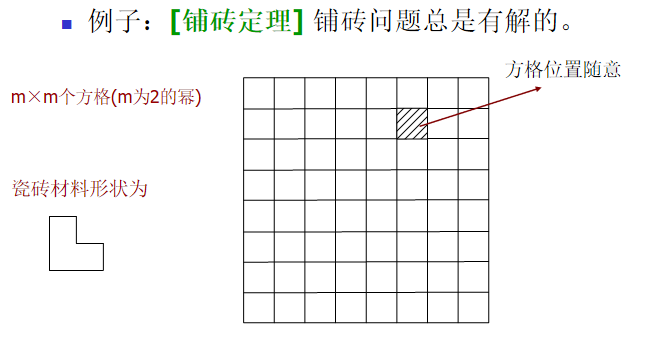
\includegraphics[width = 1\textwidth]{3.png}

\section{源码}

源码在附件中$\cdots$

\section{输出结果}

输出结果中,数字相同的连续格子表示是一块地砖。

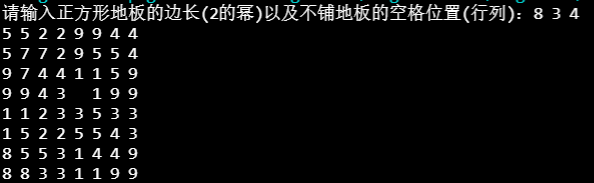
\includegraphics[width = 1\textwidth]{2.png}

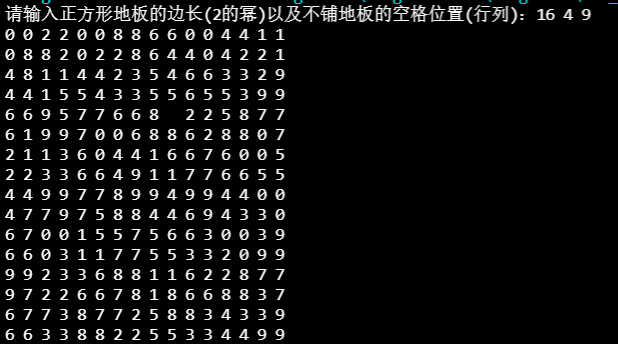
\includegraphics[width = 1\textwidth]{1.png}

\end{document}